\chapter{Реализация нейросетевых моделей для задач управления в АСУТП}

\section{Процесс пастеризации}

Для моделирования были реализованы соответствующие модули. Использовался язык С++, операционная система – Windows 7 и Linux.

Рисунок \ref{fig:Pasteurization_modeling_results} показывает результаты моделирования для следующих значений параметров $k = 525$ и $T = 450$ (см. табл. \ref{table:pasterizer_params}), $P = 0.5$, $T_I = 5$ и $T_D = 0.01$, требуемое задание \SI{20}{\celsius}.

\begin{figure}[H]
    \centering
    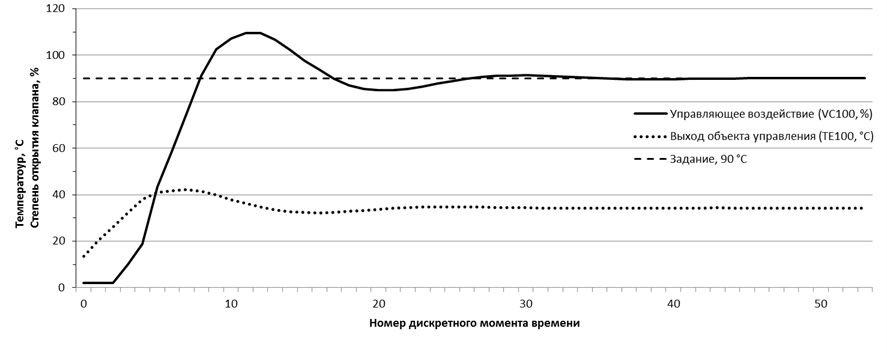
\includegraphics[width=\textwidth]{images/chapter_3/Pasteurization_modeling_results.png}
    \caption{Результаты моделирования процесса пастеризации}
    \label{fig:Pasteurization_modeling_results}
\end{figure}

Для предварительного обучения использовались сохраненные данные работы объекта управления – 50 первых точек c размером окна – 10 (рис. \ref{fig:Pasteurization_modeling_results}), точность обучения 0.00005. Если во время работы в течение 10-ти тактов времени ошибка управления превышала 2, то происходило обучение нейронной сети, точность обучения 0.0001, ограничение на количество итераций обучения – 10.

Результаты моделирования показывает рис. 3.2 и 3.3.

\begin{figure}[H]
    \centering
    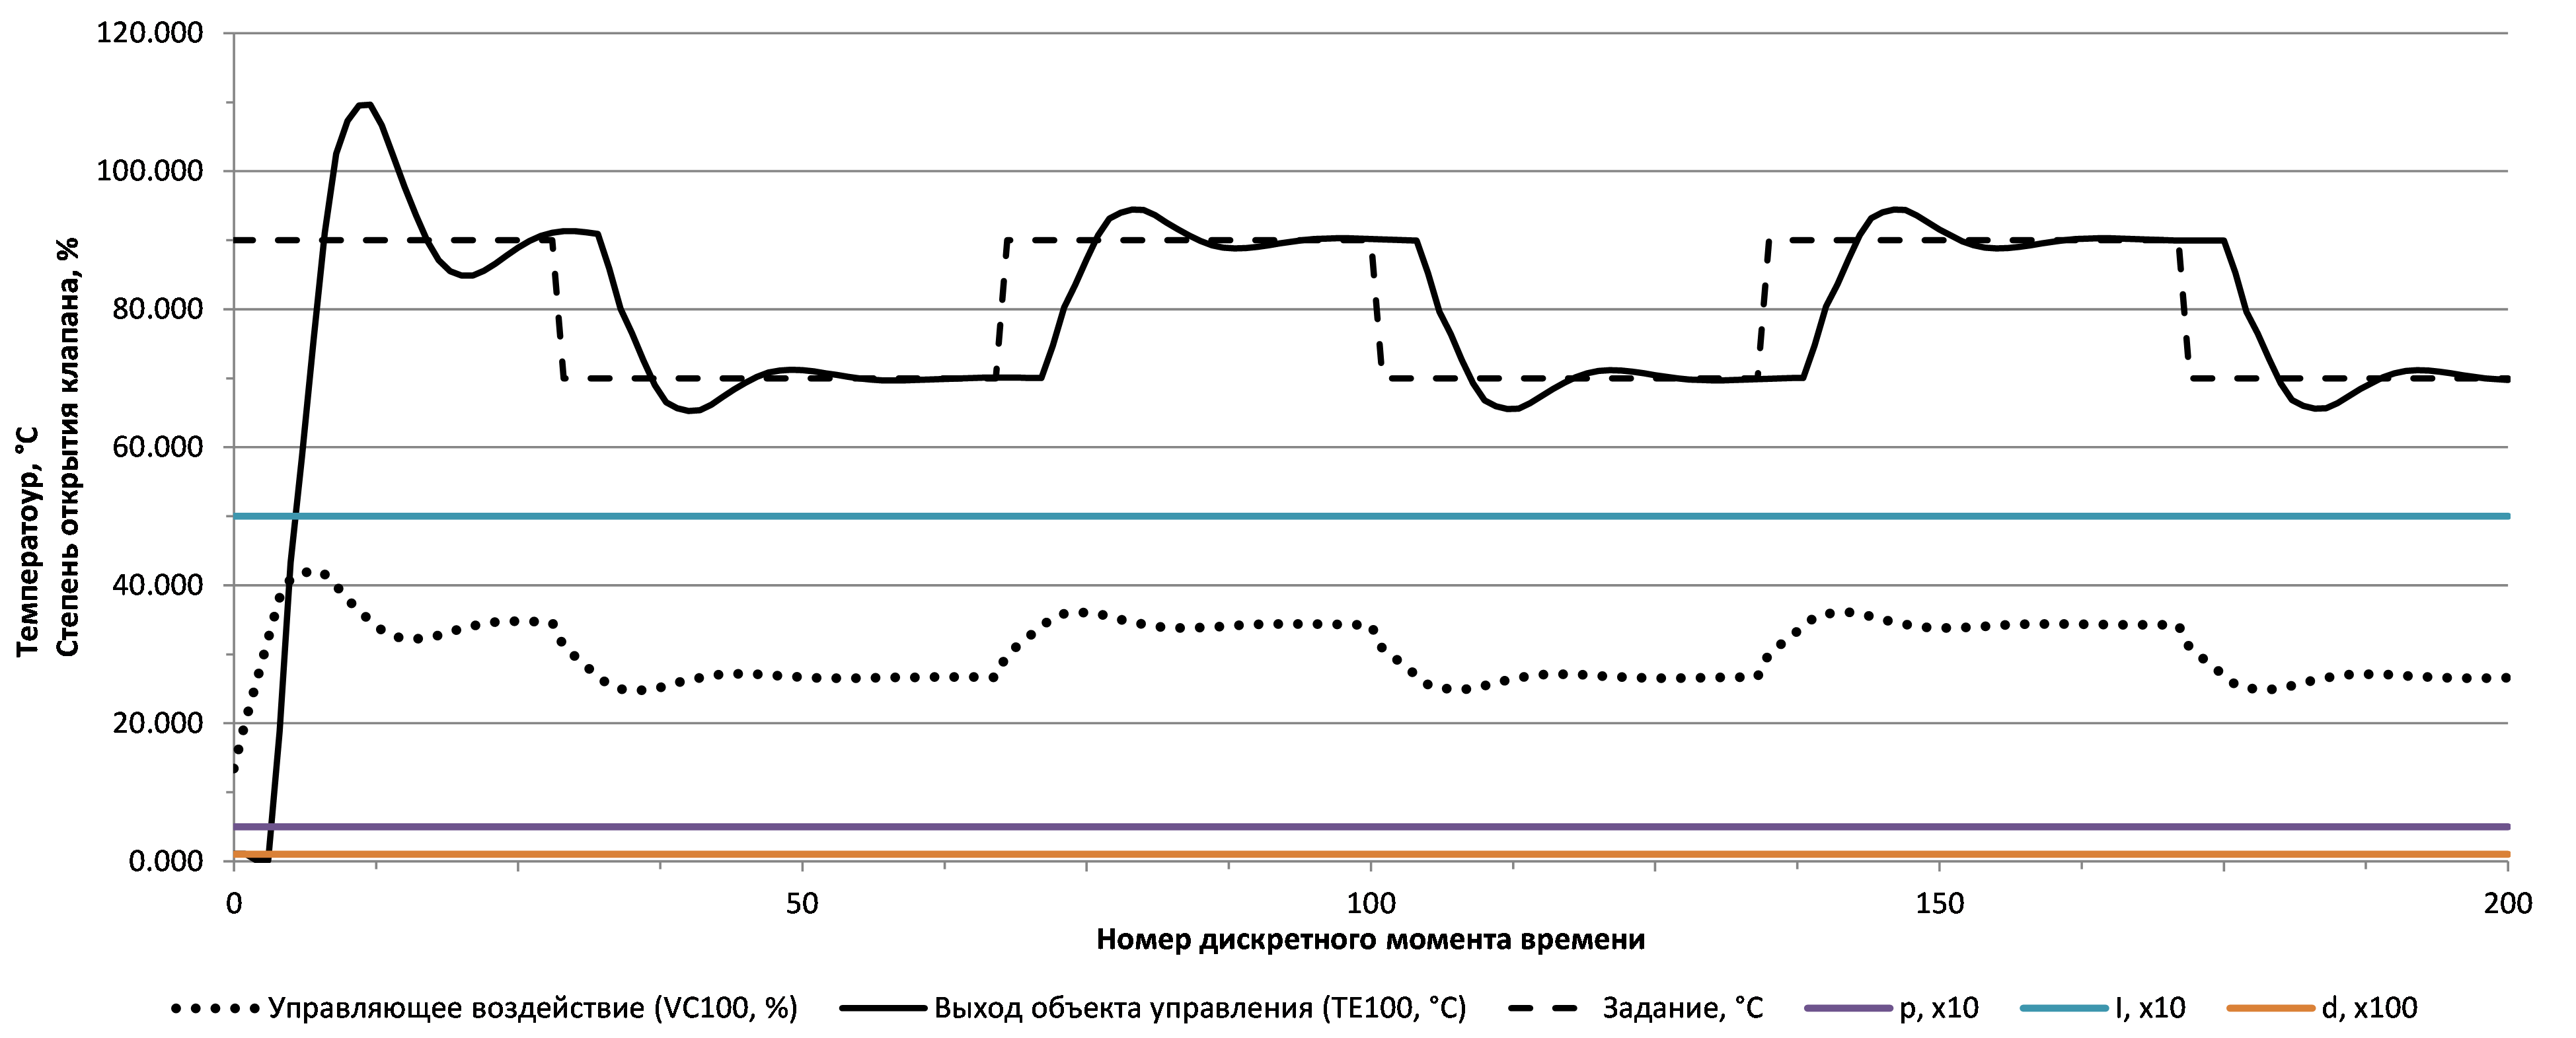
\includegraphics[width=\textwidth]{images/chapter_3/Pasteurization_modeling_results_with_typical_PID.png}
    \caption{Результаты моделирования. Работа обычного ПИД-регулятора}
    \label{fig:Pasteurization_modeling_results_with_typical_PID}
\end{figure}

Видно, что при изменении задания переходной процесс не изменяется и сохраняется один и тот же уровень перерегулирования, так как коэффициенты ПИД-регулятора статичны. Значение перерегулирования $\delta = \SI{5}{\celsius}$ (5\%).

\begin{figure}[H]
    \centering
    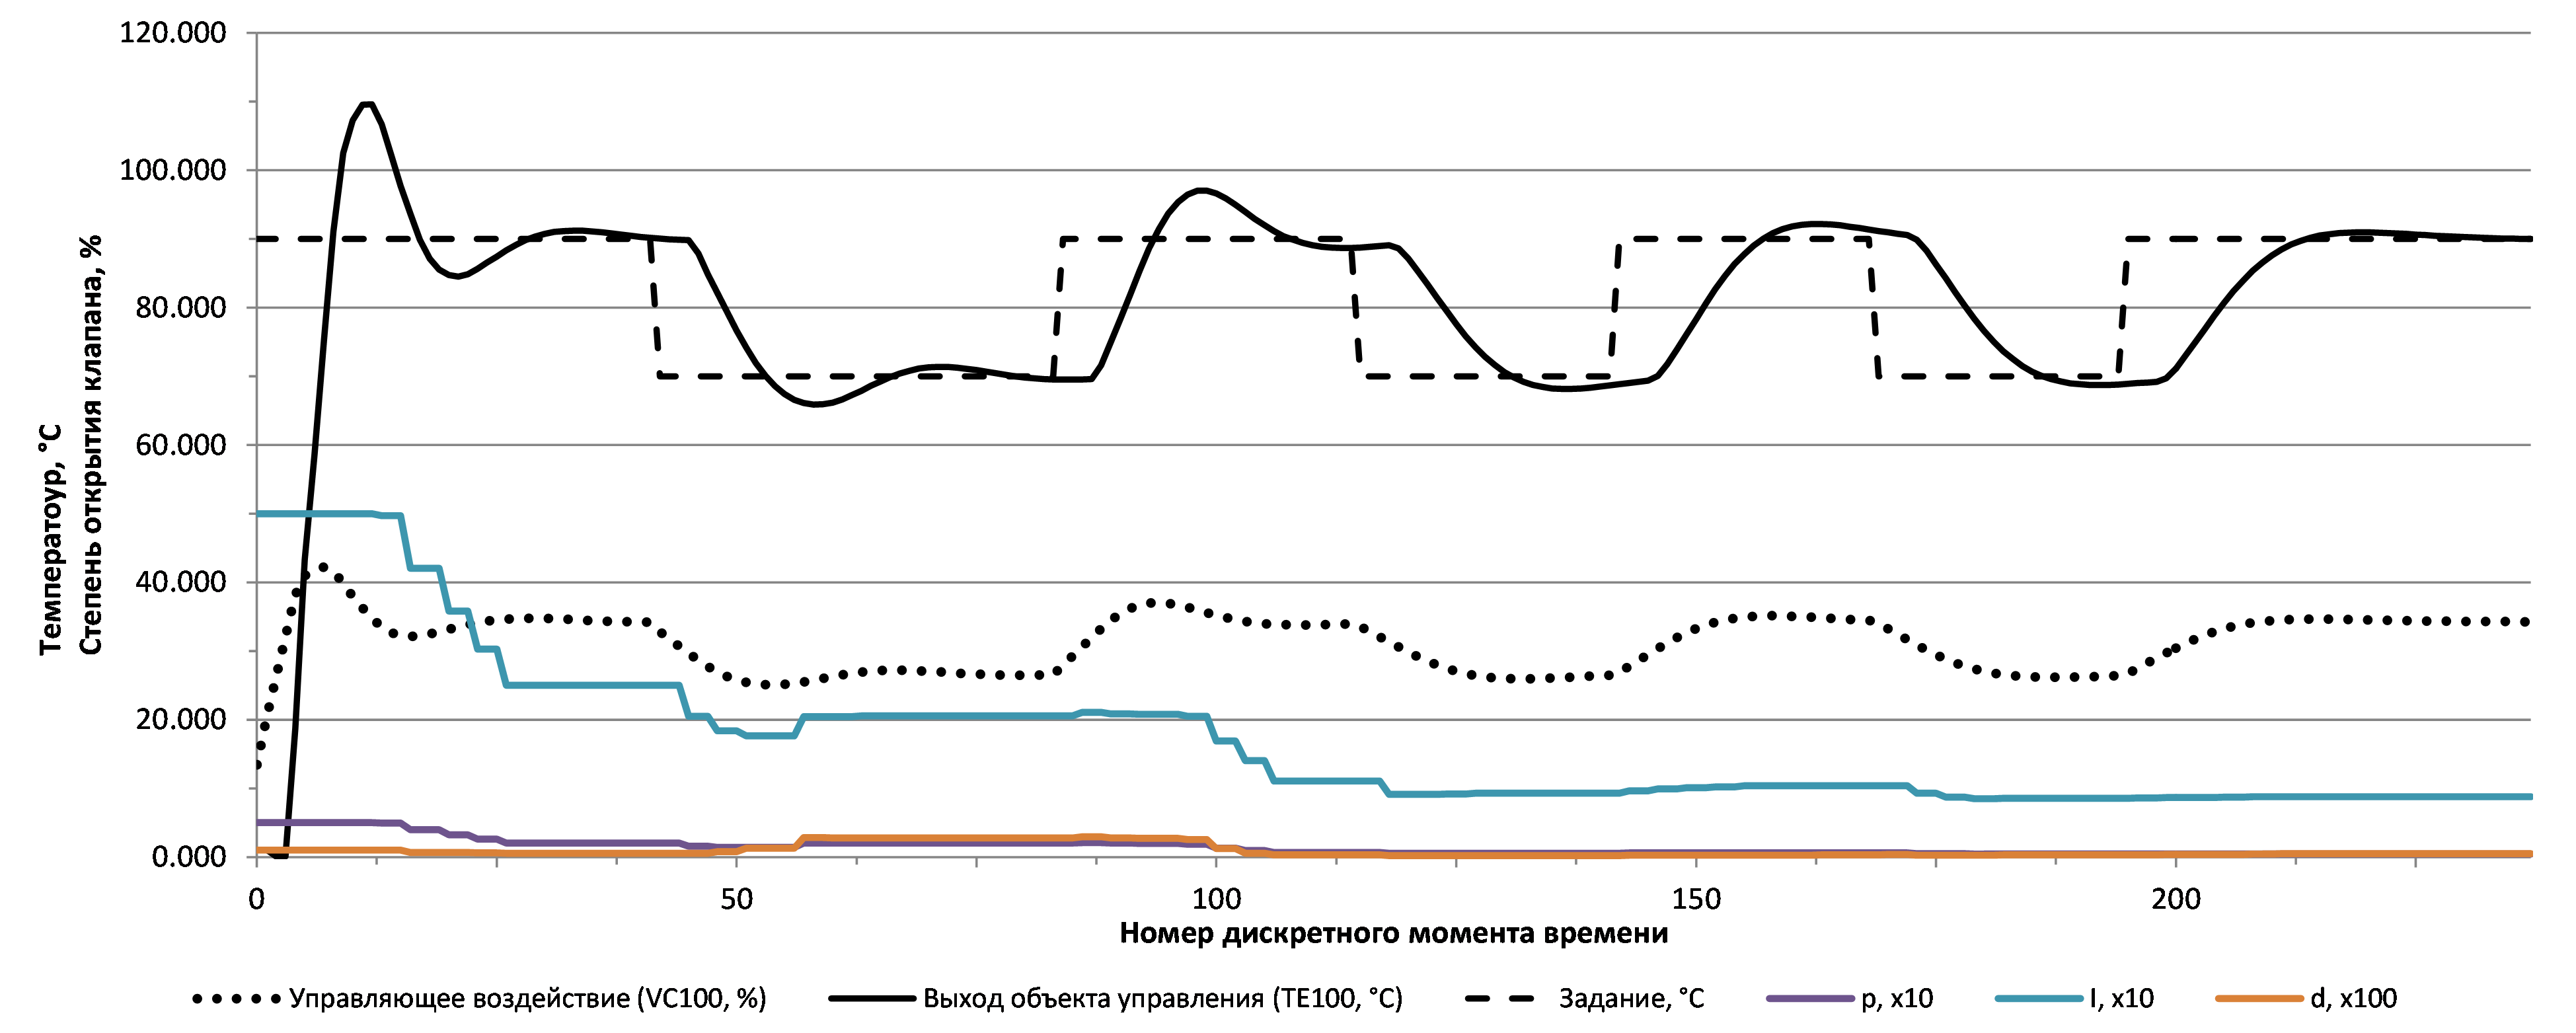
\includegraphics[width=\textwidth]{images/chapter_3/Pasteurization_modeling_results_with_neuro_PID.png}
    \caption{Результаты моделирования. Работа нейро-ПИД-регулятора}
    \label{fig:Pasteurization_modeling_results_with_neuro_PID}
\end{figure}

Можно убедиться, что при четвертом и пятом изменении задания переходной процесс улучшается. Начальные значения коэффициентов - $P = 0.5$, $T_I = 5$ и $T_D = 0.01$, после надстройки – $P = 0.43$, $T_I = 0.9$ и $T_D = 0.005$, значение перерегулирования $\delta = \SI{1}{\celsius}$ (1\%).